\documentclass{article}
\usepackage{graphicx} % Required for inserting images
\usepackage[top=0.9in, bottom=1in, left=1.5in, right=1.5in]{geometry}
\usepackage[utf8]{inputenc}
\usepackage[icelandic]{babel}
\usepackage[T1]{fontenc}
\usepackage[sc]{mathpazo}
\usepackage[parfill]{parskip}
\renewcommand{\baselinestretch}{1.2}
\usepackage{booktabs,tabularx}
\usepackage{multirow}
\usepackage{enumerate}
\usepackage{adjustbox}
\usepackage{multicol}
\usepackage{xcolor}
\usepackage{algpseudocode}
\usepackage{tikz}
\usepackage{hyperref}
\usepackage{nicefrac}
\usepackage{changepage}
\usetikzlibrary{arrows, positioning, calc, graphs}
\usepackage{amsmath, amsfonts, amssymb, amsthm}
\usepackage{graphicx}
\usepackage{tikz}
\usepackage{minted}
\usemintedstyle{manni}
\title{Tölvugrafík Heimadæmi 6 }
\author{Ragnar Björn Ingvarsson, rbi3}
\tikzset{->, >=stealth', shorten >=1pt, node distance=2cm,thick, main node/.style={circle,draw,minimum size=3em}}

\begin{document}
\renewcommand\thepage{}

	\maketitle

	\newpage
	\setcounter{page}{1}
	\renewcommand\thepage{\arabic{page}}

	\section{}
	\begin{itemize}
		\item[a)] Öfugu þríhyrningarnir birtast svo að þeir eru bara litaðir 
			með umhverfislitnum, svo það er flatur litur á þeim.
		\item[b)] Ef við kveikjum á bakhliðareyðingu (back-face culling), 
			þá hverfa bara þessir þríhyrningar.
	\end{itemize}

	\section{}
	\url{https://Skogarbjorn.github.io/h6/2/phong.html}
	\begin{center}
		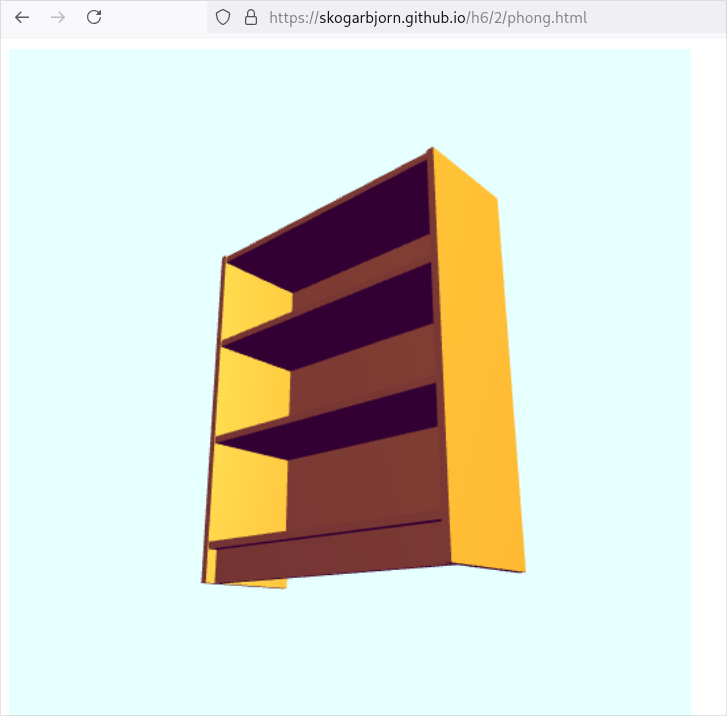
\includegraphics[width=0.75\textwidth]{billy.png}
	\end{center}

	\newpage
	\section{}
	\url{https://skogarbjorn.github.io/h6/3/tea.html}
	\begin{itemize}
		\item[a)] Hér breyti ég bara GLSL kóðanum til að, í stað þess að 
			bera alla fleti saman við $1.8$ þá ber ég þá saman við 
			uniform breytu sem ég svo tengi við javascript skránna og 
			uppfæri hana á viðeigandi hátt í hvert skipti sem ýtt er á 
			niður eða upp örina.
		\item[b)] Hér læt ég \texttt{materialAmbient} vigurinn fá gildi 
			sem er ákvarðað af \texttt{hue} breytu sem er svo notuð til að 
			reikna \texttt{rgb} gildi útfrá \texttt{hsv2rgb} fallinu, og 
			uppfæri \texttt{hue} og allt sem kemur á eftir í hvert skipti 
			sem notandi ýtir á vinstri eða hægri örina.
	\end{itemize}

	\begin{center}
		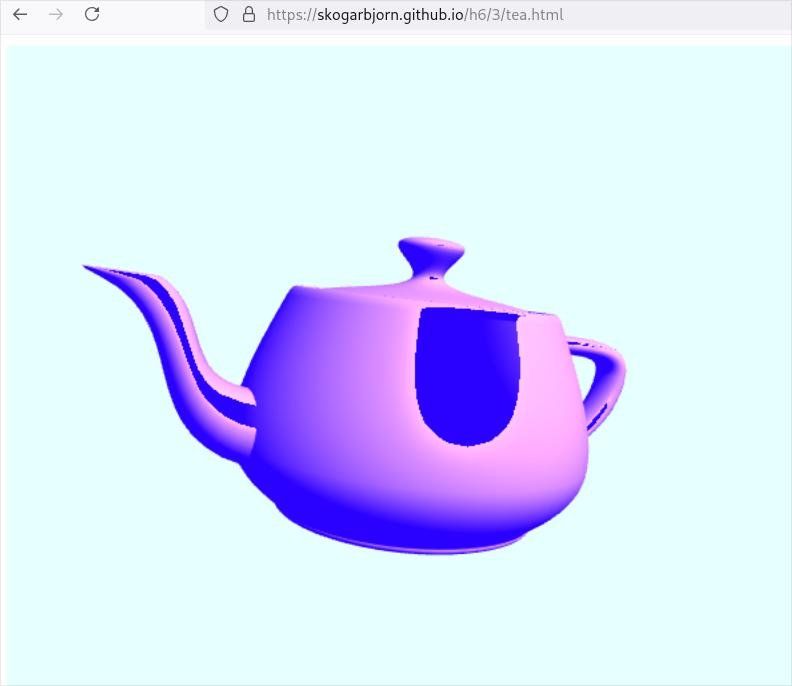
\includegraphics[width=0.75\textwidth]{tea.png}
	\end{center}

	\section{}
	\begin{itemize}
		\item[a)] Það er betra vegna þess að ef við geymum þjappaðar 
			myndir á innra minni þá taka þær í raun aukalegt pláss og tíma 
			þar sem það þarf alltaf fyrst að afþjappa þær til að sýna, 
			svo við myndum vera að eyða hraðasta minninu okkar í að alltaf 
			vera að afþjappa myndirnar, þegar við getum bara afþjappað þær 
			fyrst og svo sent þær til innra minnis.
		\item[b)] Þetta gæti verið nothæft til dæmis til að geyma mjög 
			margar myndir í innra minni á sama tíma, sem væri kannski gott 
			í sumum tilfellum, en þá kemur vandamálið að það þyrfti þá 
			alltaf að afþjappa þær til að nota, svo allt yrði í raun 
			hægvirkara í lokin.
	\end{itemize}

	\newpage
	\section{}
	\begin{itemize}
		\item[i.] Hér þarf \texttt{gl.TEXTURE\_WRAP\_S} að vera á 
			\texttt{gl.REPEAT} og \texttt{gl.TEXTURE\_WRAP\_T} að vera 
			á \texttt{gl.CLAMP\_TO\_EDGE} en mynsturhnitin bara fylkið
			\begin{verbatim}
var texCoords = [
    vec2(0.0, 0.0),
    vec2(3.0, 0.0),
    vec2(3.0, 3.0),
    vec2(3.0, 3.0),
    vec2(3.0, 0.0),
    vec2(0.0, 0.0)
];
			\end{verbatim}
		\item[ii.] Hér viljum við að mynsturhnitin séu frá $0.5$ til $2.5$ 
			í $S$ ás svo við fáum að \\ \texttt{gl.TEXTURE\_WRAP\_S} sé 
			\texttt{gl.REPEAT} og að \texttt{gl.TEXTURE\_WRAP\_T} sé einnig 
			\texttt{gl.REPEAT}. Svo eru mynsturhnitin svona:
			\begin{verbatim}
var texCoords = [
    vec2(0.5, 0.0),
    vec2(2.5, 0.0),
    vec2(2.5, 3.0),
    vec2(2.5, 3.0),
    vec2(0.5, 3.0),
    vec2(0.5, 0.0)
]
			\end{verbatim}
		\item[iii.] Hér viljum við snúa við pottinum svo við breytum bara 
			röð punktanna í fylkinu okkar,
			\begin{verbatim}
var texCoords = [
    vec2(1.0, 1.0),
    vec2(0.0, 1.0),
    vec2(0.0, 0.0),
    vec2(0.0, 0.0),
    vec2(1.0, 0.0),
    vec2(1.0, 1.0)
]
			\end{verbatim}
	\end{itemize}
\end{document}
